\chapter{Background Theory}
\label{BackgroundTheory}
\graphicspath{{Figures/BackgroundTheory/}{Figures/Common/}}


\section{Indistinguishable particles and BEC, a non-classical phenomenon}

Condensate fraction, temperature dependence

\section{Hamiltonian}

After second-quantisation, the Hamiltonian describing an interacting multi-component field of bosonic atoms is
\begin{align}
    \label{BackgroundTheory:BasicHamiltonian}
    \begin{split}
        \hat{H} &=
            \sum_i \int d \vect{x}\, \hat{\Psi}_i^\dagger(\vect{x}) \left(- \frac{\hbar^2\nabla^2}{2 M} + V_{i}(\vect{x}) \right) \hat{\Psi}_i^{\phantom{\dagger}}(\vect{x})\\
            &+ \frac{1}{2}\sum_{i j m n} \int \int d\vect{x}\, d\vect{x}'\, \hat{\Psi}_i^\dagger(\vect{x}) \hat{\Psi}_j^\dagger(\vect{x}') V_{ijmn}(\vect{x} - \vect{x}') \hat{\Psi}_m^{\phantom{\dagger}}(\vect{x}') \hat{\Psi}_n^{\phantom{\dagger}}(\vect{x}),
    \end{split}
\end{align}
where $\hat{\Psi}_i(\vect{x})$ is the bosonic annihilation operator that removes an atom in the internal state $i$ at position $\vect{x}$.  These fields obey the commutation relations
\begin{align}
    \left[\hat{\Psi}_i(\vect{x}),\, \hat{\Psi}_j(\vect{x}') \right] &= 0\\
    \left[ \hat{\Psi}_i^{\phantom{\dagger}}(\vect{x}),\, \hat{\Psi}_j^{\dagger}(\vect{x}')\right] &= \delta_{ij} \delta(\vect{x} - \vect{x}').
\end{align}
The potential $V_i(\vect{x})$ describes the external potential experienced by atoms in the internal state $i$, and will include contributions from gravity and any optical or magnetic trapping fields present.  A common example from this thesis is the cylindrically symmetric harmonic trap of the form
\begin{align}
    V(\vect{x}) &= \frac{1}{2} M \left(\omega_r^2 x^2 + \omega_r^2 y^2 + \omega_z^2 z^2 \right),
\end{align}
where $\omega_r$ is the radial trapping frequency, and $\omega_z$ is the trapping frequency in the $z$ direction.  Usually $\omega_r$ is significantly larger than $\omega_z$.  In this case, $x$ and $y$ are referred to as the `tight' trapping dimensions, and $z$ the `weak' trapping dimension.

The interatomic interaction potential $V_{ijmn}(\vect{x})$ describes scattering processes between two particles in the $m$ and $n$ internal states separated by $\vect{x}$ that scatter into the $i$ and $j$ internal states.  If the atoms have only a single internal state, this is simply the interatomic potential.

Atoms do, however, have internal structure: the quantum numbers $n$, $l$ and $m_l$ for the orbit of each electron; the projections $m_s$ for the spin of each electron; and the quantum numbers describing the state of the atom's nucleus.  Due to the couplings between these different states, none of these are `good' quantum numbers in the sense that they label eigenstates of the Hamiltonian describing a single atom.  For atoms that are well-approximated by a positively-charged core and a single orbiting electron (such as the alkali and metastable noble gas atoms used in most BEC experiments), the good quantum numbers are the principal quantum number for the primary electron $n$, the total angular momentum $F$, and its projection $m_F$ \citep{Leggett:2001}.  In practice, states with $n > 0$ decay on timescales significantly shorter than typical experimental timescales.  The $n > 0$ levels, however can contribute significantly when the atoms are driven with light near-resonant with an $n = 0 \leftrightarrow n'$ transition.  The $i$ index of the atomic field operator $\hat{\Psi}_i(\vect{x})$ is used to label the quantum numbers $n$, $F$, and $m_F$.  The notation typically used, however, differs slightly from this as $n=0$ is typically understood, and at most one of the fine-structure manifolds (which are distinguished by different values of the total electronic orbital and spin angular momentum quantum number $J$) contributes significantly.  These excited internal atomic states are usually denoted with a prime, for example $\ket{F'=1, m_F=0}$.

It is this internal atomic structure that enables atoms to be manipulated using a rich variety of techniques.  In the presence of a magnetic field, the different $m_F$ levels have different energies separated by the Zeeman splitting.  This enables atoms in certain $m_F$ levels to be trapped in a local magnetic field minimum.  In the presence of radio-frequency radiation resonant with this Zeeman splitting the $m_F$ levels within a given $F$ manifold are coupled permitting the transfer of population between levels.  In the presence of intense optical radiation far detuned from the $n=0 \leftrightarrow n'=1$ transition, depending on the polarisation, all $m_F$ levels can receive the same energy shift and be all be trapped equally.  In the presence of pairs of optical fields momentum can be coherently transferred to the atoms, and depending on the polarisations, simultaneously change their internal state.  The atom--light coupling term is discussed in detail in \sectionref{OpticalPumping:MultimodeModel}.

In the absence of additional coupling terms, the equations of motion for the atomic field operators $\hat{\Psi}_i$ are determined by the Hamiltonian \eqref{BackgroundTheory:BasicHamiltonian},
\begin{align}
    \begin{split}
    i \hbar \frac{\partial}{\partial t}\hat{\Psi}_i(\vect{x}) &= \left( - \frac{\hbar^2 \nabla^2}{2 M}  + V_i(\vect{x}) \right) \hat{\Psi}_i(\vect{x}) \\
        &+ \sum_{jmn} \int d \vect{x}'\, V_{ijmn}(\vect{x} - \vect{x}') \hat{\Psi}_j^\dagger(\vect{x}') \hat{\Psi}_m^{\phantom{\dagger}}(\vect{x}') \hat{\Psi}_n(\vect{x}).
    \end{split}\label{BackgroundTheory:NonLocalOperatorEvolution}
\end{align}
The most complicated part of this evolution is the non-local term governed by the interatomic interaction potential $V_{ijmn}(\vect{x})$.  The following section discusses an approximation in which this potential may be approximated by a \emph{local} interaction, simplifying the evolution described by \eqref{BackgroundTheory:NonLocalOperatorEvolution}.

\section{Atomic scattering}

As the composite structure of atoms is not included in \eqref{BackgroundTheory:BasicHamiltonian}, the Hamiltonian represents an effective field theory which is only valid on length scales larger than the atomic size.  At the low temperatures and densities typical of ultracold atom experiments these structures are not probed and the effective field theory is a good approximation.  Indeed, it is usual that the details of the interaction potential $V_{ijmn}(\vect{x})$ are not probed either, and the potential can be approximated by a contact interaction \citep{Leggett:2001}
\begin{align}
    V_{ijmn}(\vect{x}) &\approx U_{ijmn} \delta(\vect{x}), \label{BackgroundTheory:ContactInteractionPotential}
\end{align}
where $U_{ijmn} = 4 \pi \hbar^2 a_{ijmn}/M$, and $a_{ijmn}$ is the scattering length for the corresponding interaction.  The scattering length is chosen to reproduce the long-range scattering behaviour of the exact potential $V_{ijmn}(\vect{x})$.  Equation~\eqref{BackgroundTheory:ContactInteractionPotential} is termed the $s$-wave scattering approximation as only collisions in which the atoms have zero relative motional angular momentum occur; as the full potential has finite extent collisions with non-zero relative angular momenta (the $p$- or $d$-wave terms, for example) would occur.  These collisions have negligible amplitude at the temperatures typical of ultracold atom experiments as atoms with non-zero relative motional angular momentum cannot approach sufficiently closely for $V_{ijmn}(\vect{x})$ to be non-negligible.

In alkali atoms there are two $n=0$ $F$ manifolds, which are separated by the hyperfine splitting.  The energy difference between these two manifolds is sufficiently large that collisions between atoms in the lower manifold cannot result in any atoms being scattered into the upper manifold.  As a result of this restriction it can be shown \citep{Ho:1998} that the scattering only depends on the total angular momentum of the scattering atoms.  The interaction term of \eqref{BackgroundTheory:BasicHamiltonian} can be written as
\begin{align}
    \label{BackgroundTheory:QuasimolecularScatteringTerm}
    \hat{H}_\text{int} &= \frac{1}{2}\sum_{S, m_S}  g_S \int d \vect{x}\, \hat{\Xi}^\dagger_{S, m_S}(\vect{x}) \hat{\Xi}^{\phantom{\dagger}}_{S, m_S}(\vect{x}),
\end{align}
where $g_S = 4 \pi \hbar^2 a_S/M$ is the nonlinear interaction strength, and $a_S$ is the $s$-wave scattering length for the total hyperfine spin $S$ channel.  For bosons, the total hyperfine spin $S$ is restricted to even values due to symmetry \citep{Ho:1998}.  The quasi-molecular operator $\hat{\Xi}_{S, m_S}$ is defined in terms of the atomic annihilation operators and the appropriate Clebsch-Gordan coefficients~\citep{Ho:1998}
\begin{align}
    \hat{\Xi}_{S, m_S}(\vect{x}) &= \sum_{m_F, m_F'} \left(F, m_F; F, m_F' \middle| S, m_S \right) \hat{\Psi}_{F, m_F}(\vect{x}) \hat{\Psi}_{F, m_F'}(\vect{x}),
\end{align}
where $\left(j_1, m_1; j_2, m_2 \middle| J, M\right)$ is a Clebsch-Gordan coefficient.  For the metastable noble gases, the interaction term is also in the form of \eqref{BackgroundTheory:QuasimolecularScatteringTerm} as only one $F$ manifold is accessible.  In metastable Helium the scattering lengths $a_S$ differ by 25\%.  The consequences of this difference are considered in \chapterref{Peaks}.  For $\nucl{87}{}{Rb}$, however, the scattering lengths for collisions between $F=1$ atoms differ by at most 1\% \citep{Kempen:2002}, permitting the approximation $g_0 \approx g_2$.  The nonlinear interaction Hamiltonian can then be written in the simple form
\begin{align}
    \label{BackgroundTheory:SimpleScattering}
    \hat{H}_\text{int} &= \frac{1}{2} \sum_{ij} U_\text{int} \int d \vect{x}\, \hat{\Psi}_i^\dagger(\vect{x}) \hat{\Psi}_j^\dagger(\vect{x}) \hat{\Psi}_j^{\phantom{\dagger}}(\vect{x}) \hat{\Psi}_i^{\phantom{\dagger}}(\vect{x}).
\end{align}

When interatomic scattering is well-described by the simple interaction \eqref{BackgroundTheory:SimpleScattering}, the operator evolution of \eqref{BackgroundTheory:NonLocalOperatorEvolution} may be simplified to
\begin{align}
    i \hbar \frac{\partial}{\partial t} \hat{\Psi}_i(\vect{x}) &= \left( -\frac{\hbar^2 \nabla^2}{2 M} + V_{i}(\vect{x}) + U_\text{int} \sum_{j} \hat{\Psi}_j^\dagger(\vect{x}) \hat{\Psi}_j^{\phantom{\dagger}}(\vect{x}) \right) \hat{\Psi}_i^{\phantom{\dagger}}(\vect{x}). \label{BackgroundTheory:LocalOperatorEvolution}
\end{align}
While the approximation made to the nonlinear interaction term of the Hamiltonian has made these equations local, they cannot be solved exactly.  In the absence of the nonlinear term the atoms do not interact with one another, and the energy eigenstates do not depend on the number of atoms in the system.  In this case the field operator $\hat{\Psi}_i$ may be decomposed as
\begin{align}
    \hat{\Psi}_i(\vect{x}, t) &= \sum_j \hat{a}_{ij} \phi_{ij}(\vect{x}, t),
\end{align}
where the $\phi_{ij}$ are a set of orthogonal basis functions obeying
\begin{align}
    i \hbar \frac{\partial }{\partial t} \phi_{ij}(\vect{x}, t) &= \left( - \frac{\hbar^2 \nabla^2}{2M} + V_i(\vect{x}) \right) \phi_{ij}(\vect{x}, t),
\end{align}
and $\hat{a}_{ij}$ are stationary bosonic annihilation operators for the corresponding single-particle modes.  

With the addition of the nonlinear interaction term, the evolution of the field operator may not be decomposed into the sum of \emph{stationary} bosonic annihilation operators and time-dependent basis functions; the evolution of each `mode' would necessarily depend on the occupation of the other modes.  It is this complication that makes \eqref{BackgroundTheory:LocalOperatorEvolution} difficult to solve in the general case, either analytically \emph{or numerically}.  The difficulty numerically is the sheer amount of information needed to describe $\hat{\Psi}(\vect{x})$.  For a system with exactly $N=100$ atoms that can each occupy one of $m = 100$ spatial modes, $\sim 10^{117}$ complex numbers are needed to describe $\hat{\Psi}(\vect{x})$.  Typical BEC's have $N \gtrsim 10^5$.  While it is this complexity that it is hoped that quantum computers can harness, it is what makes it hard to solve many-body interacting quantum problems with classical computers.

The following section discusses a limit in which the field operator can be approximated by a complex function, whose evolution can feasibly be simulated numerically.

\section{Gross-Pitaevskii equation}



Briefly mention an approach to spontaneous symmetry-breaking.  This is in terms of assuming a given phase.

Derive the GP equation.  Simply, not too much fuss.  Note that the only term where an approximation is made is the scattering term.  The atom--light coupling term also suffers this problem if present, even with the RWA.

\subsection{Thomas-Fermi approximation}

Derive the TF, show a few plots or something.  Do it simply.  Apply it to outcoupling in the TF limit to determine the difference in behaviour of Rb and He* atom lasers.

\subsection{Application: Transverse profile of the atom laser}

Quick example calculation, show some pretty pictures.  Good agreement with experiment, yada yada.

\section{Density matrices and loss}
The decoherence superoperator arises naturally due to system--bath coupling of a certain form.  Gives rise to the Lindblad form, which gives rise to a certain form for a general bath occupation, and a simpler form with vacuum bath (usual case).  Show that the decoherence superoperator gives rise to usual forms for loss in expectation values.

Brief applications to spontaneous emission (assume \emph{both} the atomic ground states and photon modes are in vacuum states) and Penning ionisation.

\section{Phase-space methods}

Fokker-Planck equations derived from master equations using operator correspondences.  Given certain conditions, these can then be transformed into SDEs, which may be efficiently simulated (see \sectionref{PenningIonisationAppendix:FokkerPlanckToSDEs}).  Truncation is necessary to give rise to the TW method.  Mention validity and reproduce some of my pretty Wigner vs Truncated Wigner pictures.  

This does not rely on truncating a cumulant-expansion, but does assume that particles act independently of one-another, and only depend on a finite set of moments. (FIXME: Get a clearer picture of the difference)

\section{Other methods beyond the mean field}

Rely on truncating a cumulant expansion.

\section{Numerical Techniques}
\subsection{Absorbing boundary layers}
\subsection{Error checking}
\subsection{New piece of software}
Feature list given in \appendixref{ToolsAppendix}.

\section{Summary}
And now, on with the show!
\hrule


\section{Phase-space methods}
\label{BackgroundTheory:PhaseSpaceMethods}
%Focus primarily on truncated Wigner.

\section{Absorbing boundary layers for Schrödinger-type equations}
\label{BackgroundTheory:AbsorbingBoundaryLayers}


To solve any partial differential equation numerically, it must be restricted to a finite domain with boundary conditions imposed at the edges\footnote{This requirement can be avoided when the solution's asymptotic behaviour is known \emph{a priori}, however this case will not be encountered in this thesis.}. For some systems, this poses no additional restriction over the original problem as they are explicitly defined over a finite domain and with the correct boundary conditions this constitutes the problem itself (for example electromagnetic wave propagation in a waveguide). Other systems are naturally restricted to a finite domain (for example a BEC in a trap) and will be unaffected by the imposition of the artificial boundary conditions. 

With the exception of systems defined over a finite domain, the choice of boundary conditions at the edges of the computational domain is an artificial one; while in many cases they permit physical interpretation, this interpretation does not usually correspond to the reality of the system under consideration. As an example, consider the case of a BEC freely falling under gravity. The natural domain for this problem is infinite, but to solve this system numerically it must be restricted to a finite domain. If periodic boundary conditions are used, when the BEC falls of the bottom of the computational domain, it will reappear at the top of the domain to continue falling. If the wavefunction or its derivative is set to zero on the boundary then the BEC will reflect from the bottom of the domain. Each choice of boundary condition gives different results and none correspond to the correct behaviour in which the BEC would simply fall out of the computational domain. A strategy is therefore needed to limit the effect of the choice of the boundary conditions on the solution.

A first simple strategy would be to choose the computational domain to be large enough such that no part of the atom laser beam will reach the edge of the domain over the time of interest. While effective, this strategy can be computationally expensive and is particularly demanding in the presence of gravity. Under the influence of gravity a classical particle starting from rest will travel a distance $d = \frac{1}{2}g t^2$ in time $t$. Hence the size of the computational domain must increase as $t^2$. The spatial grid separation cannot remain constant however. As the velocity of the classical particle increases as $v = gt$, the mean wavelength of the particle $\displaystyle \lambda = \frac{\hbar}{Mv}$ must then decrease as $t^{-1}$.  To resolve the spatial dynamics of the atom laser, the step size between points must then decrease as $t^{-1}$. These two effects combine to give the scaling that the total number of spatial grid points required $N_\text{pts} \propto t^3$. Choices of uniform or variable spacing for the grid will only differ by an overall constant factor in the number of points required by this strategy; such choices cannot change the overall scaling. A different strategy is needed.

In many circumstances it is the Bose-Einstein condensate and the outcoupling process that produces the atom laser that are of interest. In such situations the remainder of the atom laser that can no longer directly interact with the BEC must be prevented from doing so as a result of its unphysical interactions with the artificial boundary conditions. The solution used in the aforementioned strategy was to continue to model the atom laser, however this is not necessary. An alternative solution is to remove this part of the atom laser from the simulation in a way that has no effect on the BEC and the outcoupling process. One strategy that takes this approach is to add an \emph{absorbing boundary layer}~\citep{Kosloff:1986,Neuhasuer:1989} between the domain of interest and the artificial boundary conditions. This absorbing boundary layer takes the form of a negative imaginary potential, which must be chosen to be deep enough to strongly attenuate any wave traversing it and smooth enough to make the probability of reflection negligible. \figureref{BackgroundTheory:AbsorbingBoundarySchematic} illustrates this strategy. Through the use of an appropriate absorbing boundary layer, the computational domain used to solve the system need not change and the scaling problem discussed previously will not occur.

\begin{figure}
    \centering
    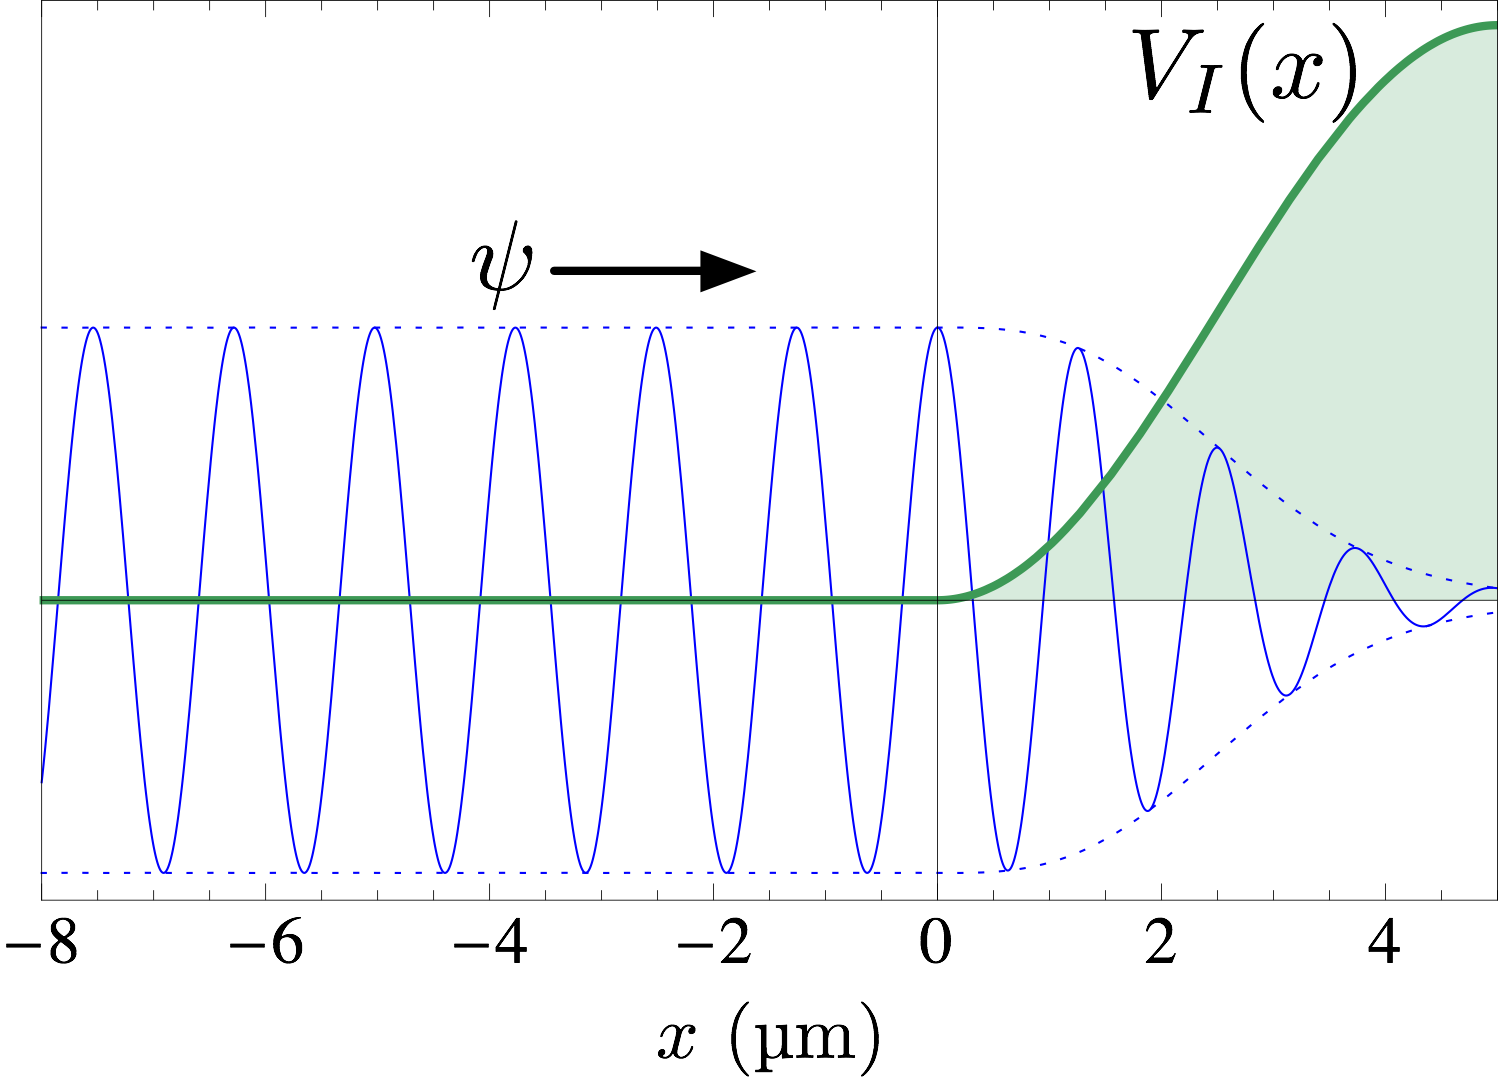
\includegraphics[width=8cm]{AbsorbingBoundarySchematic}
    \caption{
        \label{BackgroundTheory:AbsorbingBoundarySchematic}
        Schematic diagram illustrating the use of an absorbing boundary layer. A right-travelling wave is incident on the absorbing boundary layer which is given by the potential $V(x) = -i V_I(x)$. The wave is attenuated as it crosses the absorbing boundary layer.
    }
\end{figure}

An absorbing boundary layer of finite thickness can only be effective over a finite range of incident wavenumbers. Incident wavefunctions with large wavelengths (low wavenumbers) will be reflected from the absorbing boundary layer due to the rapid variation in the potential over a wavelength. Incident wavenumbers with very short wavelengths (high wavenumbers) will be transmitted through the absorbing boundary layer due to the finite amount of time spent in the absorbing boundary layer by any point on the phase-front.  Using this argument~\citet{Neuhasuer:1989} showed that the approximate range of wavenumbers over which an absorbing boundary layer will be effective is
\begin{align}
    \label{BackgroundTheory:AbsorbingBoundaryKEffectiveRange}
    \left( \frac{M \overline{V_I}}{\hbar^2 \Delta x}\right)^{\frac{1}{3}} \ll k \ll \frac{4 M \overline{V_I} \Delta x}{\hbar^2},
\end{align}
where $\overline{V_I}$ is a representative value of $V_I(x)$. The maximum and minimum limits for the wavenumber are respectively due to the requirements of negligible transmission and reflection. Although cast in terms of the wavenumber, \eqref{BackgroundTheory:AbsorbingBoundaryKEffectiveRange} is equivalent to (26) in~\citep{Neuhasuer:1989}. While not its purpose, \sectionref{MethodsAppendix:MomentumDensityFluxExampleCalculation} demonstrates how to calculate the reflection and transmission coefficients as a function of wavenumber for arbitrary absorbing boundary layers.

The use of absorbing boundary layers must be slightly modified for use in phase-space methods such as those discussed in \sectionref{BackgroundTheory:PhaseSpaceMethods}. In these cases simply adding an absorbing boundary layer to the potential would lead to unphysical results as the absorbing potential would not discriminate between real particles in a mode and the virtual particles which represent the fundamental vacuum fluctuations inherent in the field. An appropriate way of handling this problem is to add a position-dependent loss term to the master equation of the form
\begin{align}
    \label{BackgroundTheory:PhaseSpaceAbsorbingBoundaryLayer}
    \frac{d \hat{\rho}}{dt} &= \int d \vect{x}\, \frac{2}{\hbar}V_I(\vect{x})\mathcal{D}[\hat{\Psi}(\vect{x})]\hat{\rho},
\end{align}
where $\mathcal{D}$ is the usual decoherence superoperator. This master equation term leads to the same imaginary potential term in the equations of motion for the field operator with an additional noise term the for Truncated Wigner and Q function methods that restores the vacuum fluctuations that would otherwise be lost.

\parasep

In most of this thesis it is only the immediate vicinity of the BEC that is under consideration and absorbing boundary layers are used to restrict the computational domain to this region.  As the use of absorbing boundary layers is a technical issue not related to the underlying physics, they are not included in equations of motion given in this thesis but should be understood to be included when simulations are performed.  

While direct application of absorbing boundary layers permit the study of dynamics near the BEC, in \chapterref{TransverseProfile} the transverse profile of the atom laser a large distance from the BEC is considered.  In this case a different strategy must be used to avoid the $N_\text{pts} \propto t^3$ scaling discussed above.  Such a strategy is discussed in \sectionref{TransverseProfile:DropGP}.

\section{Spontaneous symmetry-breaking and all that}
\label{BackgroundTheory:SymmetryBreaking}

Quantum-mechanics is \emph{linear}. If my system is in the state $\displaystyle \hat{\rho} = \sum_i P_i \ketbra{\Psi_i}{\Psi_i}$, then I can simply consider the evolution of each of the $\displaystyle \rho_i = \ketbra{\Psi_i}{\Psi_i}$ \emph{individually} and then construct the weighted average for any expectation value that I'm interested in $\mean{\hat{O}} = \sum_i P_i \bra{\Psi_i}\hat{O}\ket{\Psi_i}$. Hence, the problem of `there is no mean field' is meaningless, as we can never measure the quantity $\mean{\hat{\Psi}}$, it is only ever number-conserving operators that are physically meaningful for atoms. Because of all this, the state $\hat{\rho} = \ketbra{\Psi}{\Psi}$ where $\ket{\Psi}$ is a coherent state is physically \emph{indistinguishable} from the state $\displaystyle \hat{\rho} = \frac{1}{2\pi}\int d\phi\, \ketbra{\Psi e^{i\phi}}{\Psi e^{i\phi}}$. Hence I can make my damned mean-field approximation if I want to. And I won't hear any complaints that it is `unphysical'. Some useful papers~\citep{Leggett:1991fj,Molmer:1997fr}

\section{Truncated Wigner}
\label{BackgroundTheory:TruncatedWigner}
We must talk about the initial state noise being interpreted as `virtual' particles. The exact number required due to the vacuum energy of the harmonic oscillator.
Operator correspondences must be described here.
\section{Rubidium}
\label{BackgroundTheory:Rubidium}
\section{Metastable helium}
\label{BackgroundTheory:Helium}

\begin{table}
    \centering
    \begin{tabular}{cc}
    \toprule
    Parameter & Value\\
    \midrule
    Quasimolecule $S=0$ scattering length & $a_{S=0}=\unit[9.46]{nm}$\\
    Quasimolecule $S=2$ scattering length & $a_{S=2}=\unit[7.51]{nm}$\\
    Penning ionisation rate & $\Kunpol = \unit[7.7\times 10^{-17}]{m\textsuperscript{3}}$\\
    \bottomrule
    \end{tabular}
    \caption{\label{BackgroundTheory:He*Parameters} Relevant parameters of metastable helium.}
\end{table}

\subsection{Penning ionisation}
\label{BackgroundTheory:PenningIonisation}

The primary attraction of creating Bose-Einstein condensates of metastable helium atoms is that their large internal energy ($\unit[20]{eV}$) enables single-atom detection with high spatial (\micro m) and temporal resolution (ns). However, this large internal energy can be released when two metastable helium atoms collide resulting in Penning ionisation (PI),
\begin{align}
    \label{BackgroundTheory:PenningIonisation}
    \text{He}^* + \text{He}^* & \rightarrow \left\{
        \begin{matrix}
            \text{He}^+ + \text{He} + e^-\\
            \text{He}_2^+ + e^-
        \end{matrix}\right.
\end{align}
While this process dominates for unpolarised cold samples such as magneto-optical traps~\citep{Bardou:1992}, it does not prohibit the formation of Bose-Einstein condensates as the process is suppressed by five orders of magnitude~\citep{Shlyapnikov:1994} in polarised samples.  This suppression is due to conservation of angular momentum. While the reactants each have a total angular momentum $s=1$, giving their combined total angular momentum as either $S=0$ or $S=2$ (assuming $s$-wave collisions), the products each have total angular momentum $s=\frac{1}{2}$ (in the case of $\text{He}^+$, $e^-$ and $\text{He}_2^+$) or $s=0$ (for $\text{He}$), giving the total angular momentum of the products as either $S=0$ or $S=1$. Hence spin polarised states having $S=2$, $m_S=\pm2$ cannot directly undergo the process \eqref{BackgroundTheory:PenningIonisation}.

In general as $S$ is conserved, any of the $S=2$ quasimolecule states will be prevented from directly undergoing Penning ionisation. As collisions with nonzero relative angular momentum can be neglected at BEC temperatures~\citep{Venturi:2000,Stas:2006kx} (due to the atoms having insufficient energy to penetrate the centrifugal barrier), it is only the $S=0$ quasimolecule state that undergoes Penning ionisation.

As derived in \sectionref{PenningIonisationAppendix:MasterEquation} the master equation term describing Penning ionisation is
\begin{align}
    \left.\frac{d \hat{\rho}}{dt}\right|_\text{PI} &= \frac{9}{2} \Kunpol \int d \vect{x}\, \mathcal{D}\left[ \hat{\Xi}_{S=0, m_S=0}\right] \hat{\rho},
\end{align}
where $\Kunpol = \unit[7.7\times 10^{-17}]{m\textsuperscript{3}s\textsuperscript{-1}}$ is the rate constant for the production of ions due to Penning ionisation in an unpolarised thermal sample at $\unit[1]{\micro K}$~\citep{Stas:2006kx}, and the $S=0$ quasimolecule state that undergoes Penning ionisation is given by
\begin{align}
    \hat{\Xi}_{S=0, m_S=0} &= \frac{1}{\sqrt{3}} \left( 2 \hat{\Psi}_1 \hat{\Psi}_{-1} - \hat{\Psi}_0 \hat{\Psi}_0\right).
\end{align}

\section{Pumping and (atom) lasers}
\label{BackgroundTheory:Lasers}
A brief overview of what gives a laser its properties. Refer to Wiseman's paper~\citep{Wiseman:1997ba} and compare the optical and atom lasers. Alternatives for the irreversibility / source are discussed in \chapterref{OpticalPumping,KineticTheory}.

There are two fundamental reasons making the pumping of an atom laser harder than pumping an optical laser is that the dispersion relation for potential reservoirs is not flat by comparison to the dispersion relation for atoms.  For an optical laser in the homogeneous broadening limit, \emph{all} atoms in the sample can contribute to gain.  Fundamentally this is because independent of what momentum the atom might have, it can still be stimulated to emit a photon into the lasing mode as the decay rates of the excited and/or ground atomic states are greater than any possible energy detuning in this process.  The second fundamental issue affecting atom lasers is that atom number is conserved.  It is therefore inescapable that there will be atoms in a (potentially) non-condensed source mode in the vicinity of the lasing mode.  Unless a Feschbach resonance is used to set the scattering-length of atomic interactions to zero, the atoms in the source mode will disrupt the phase stability of the lasing mode.

In \chapterref{OpticalPumping}, we attempt to solve the first problem by making the momentum distribution of source atoms sufficiently narrow that it can be guaranteed that every atom will be momentum-resonant with the pumping process at some point.  In \chapterref{KineticTheory}, we use atomic modes as the reservoir.  Although their dispersion relation cannot be flat with respect to that of the atoms in the source mode, it is at least far more comparable than that of light (which is used in \chapterref{OpticalPumping}).

Ideally we should pump an atom laser using something with a flat dispersion relation.  One possibility that comes to mind is the phonon.  However it is necessary that the reservoir is essentially a pure vacuum.  Phonons produced in a condensate cannot escape the system unless the system is in contact with other atoms.  If these other atoms are thermal, than it will have its own phonons which will propagate into the condensate.  If the condensate is not in physical contact with anything, then the phonons cannot leave the system: there is no evaporation process for phonons.

Stolen from \citep{Ballagh:2000oq}:
Despite the parallels with optical laser theory, the fundamental differences between photons and atoms remain important. They arise principally because atoms have rest mass, and because they interact with each other. Unlike photons, atoms cannot be created or destroyed, rather they are transferred into the laser mode from some other mode. The interactions produce phase dynamics, which degrades the coherence of the atom laser, and self repulsion which spreads the output beam and limits the possible focussing. Even when these interactions are neglected, atoms have dispersive propagation in vacuum.
